\documentclass[conference]{IEEEtran}

\usepackage{amsmath}
\usepackage{graphicx}
\usepackage{booktabs}
\usepackage{array}
\usepackage{multirow}
\usepackage{url}

\title{MiNAE: Patient-Level Validation and Technical Audit of Public Cell-Free DNA Fragmentomics for Hepatocellular Carcinoma Detection}

% Author information is intentionally omitted for IEEE BIBM 2026 double-blind review.
\author{}

\begin{document}

\maketitle

\begin{abstract}
Early detection of hepatocellular carcinoma (HCC) remains difficult because standard surveillance tools have limited sensitivity in high-risk liver disease populations. Cell-free DNA (cfDNA) fragmentomics has emerged as a promising noninvasive signal for cancer detection, but public-data reproducibility, leakage-free validation, and technical confounding remain important challenges. This study presents MiNAE, a reproducible machine learning framework that evaluates whether cfDNA fragment-size architecture can distinguish HCC from chronic liver disease controls using public FinaleDB fragment-coordinate files. MiNAE converts compressed fragment coordinates into normalized fragment-size features, compares hg38 and hg19 global feature spaces, evaluates dual-reference fusion and chromosome-targeted feature strategies, and uses patient-level train, test, and final validation splits to prevent leakage across genome builds. In a locked held-out validation split of 40 patients, a dual-reference linear support vector machine achieved an ROC-AUC of 0.900, accuracy of 0.875, sensitivity of 0.850, specificity of 0.900, and precision of 0.895 for HCC versus cirrhosis and hepatitis B controls. Across 100 repeated held-out validations, hg38 global fragmentomics showed the most stable mean performance, with mean ROC-AUC of 0.889 and mean accuracy of 0.816. External liver-disease fragment-length replication achieved ROC-AUC 0.891 but also showed strong technical-covariate signal, reinforcing the need for batch-aware validation. These results support cfDNA fragmentomics as a promising computational biomarker signal for HCC research while emphasizing that MiNAE is a retrospective validation framework, not a clinically validated diagnostic.
\end{abstract}

\begin{IEEEkeywords}
cell-free DNA, fragmentomics, hepatocellular carcinoma, machine learning, liquid biopsy, bioinformatics, FinaleDB
\end{IEEEkeywords}

\section{Introduction}
Hepatocellular carcinoma (HCC) is a major cause of cancer mortality, and early detection is clinically important because treatment options and survival are strongly stage-dependent. Current surveillance approaches, including ultrasound and alpha-fetoprotein (AFP), are imperfect, particularly in patients with cirrhosis or viral hepatitis \cite{tzartzeva2018surveillance}. This creates a need for noninvasive biomarkers that can detect HCC in clinically realistic high-risk populations rather than only separating cancer from healthy controls.

Liquid biopsy methods often focus on circulating tumor DNA mutations, methylation, or copy-number alterations. These approaches can be powerful, but mutation detection may require deep sequencing when tumor fraction is low. cfDNA fragmentomics provides a complementary strategy by analyzing the physical properties of DNA fragments released into plasma. Because cfDNA fragmentation is influenced by nucleosome positioning, chromatin accessibility, nuclease activity, and cell death processes, fragment-size patterns can provide information about tissue state and disease biology \cite{snyder2016cellfree,mouliere2011fragmentation,cristiano2019genomewide}.

Prior studies have shown that genome-wide cfDNA fragmentomics can detect multiple cancers, including HCC \cite{cristiano2019genomewide,foda2023detecting}. The aim of MiNAE is therefore not to claim that cfDNA fragmentomics for HCC is a new biological concept. Instead, this study asks a narrower computational question: can an open, reproducible, patient-level fragmentomics pipeline built from public coordinate-level data recover HCC signal against chronic liver disease controls while explicitly auditing feature strategies, split sensitivity, and technical confounding?

The main contributions are:
\begin{itemize}
    \item a reproducible pipeline that converts FinaleDB fragment-coordinate files into normalized fragment-size features without using raw genomic sequences;
    \item a patient-level validation design that prevents leakage across hg38 and hg19 reference builds;
    \item an ablation study comparing hg38 global, hg19 global, dual-reference fusion, chromosome-targeted fusion, and combined feature strategies;
    \item a robustness audit using 100 repeated held-out validations, permutation testing, error analysis, and a technical-feature negative control.
\end{itemize}

This framing is intentionally conservative. MiNAE is not presented as a new clinical diagnostic test, and the experiments do not replace prospective clinical validation. Instead, the contribution is a transparent computational validation study designed to test whether public coordinate-level cfDNA fragmentomics can recover a biologically plausible HCC signal under leakage-aware validation.

\section{Related Work}
cfDNA fragmentation has a biological basis in chromatin structure and nuclease-mediated DNA cleavage. Snyder et al. showed that cfDNA contains nucleosome-footprint information that can inform tissue of origin \cite{snyder2016cellfree}. Cancer-derived cfDNA is often shorter than non-tumor cfDNA, motivating the use of short-to-long fragment ratios and genome-wide fragmentation patterns as cancer biomarkers \cite{mouliere2011fragmentation,cristiano2019genomewide}.

The DELFI framework demonstrated that genome-wide cfDNA fragmentation features from shallow whole-genome sequencing can classify cancer states \cite{cristiano2019genomewide}. Foda et al. later evaluated whole-genome cfDNA fragmentomes for liver cancer detection across average-risk and high-risk groups, reporting strong sensitivity and specificity for HCC detection \cite{foda2023detecting}. These studies establish the biological and clinical relevance of fragmentomics for HCC.

Public reproducibility remains challenging because raw cfDNA sequencing datasets are often controlled-access. FinaleDB addresses this by providing uniformly processed, de-identified fragment-coordinate datasets across multiple diseases and genome builds \cite{zheng2021finaledb}. Additional public fragmentomics resources, including the Annapragada et al. liver disease fragmentome repository, make it possible to evaluate external fragment-length replication without downloading raw sequencing files \cite{annapragada2026cirrhosis}. MiNAE uses public data substrates and focuses on transparent validation, feature ablation, and technical auditing rather than clinical deployment.

This study differs from prior HCC fragmentomics work in three ways. First, it uses only public fragment-coordinate files rather than raw protected sequence data. Second, it evaluates the same patients across hg19 and hg38 without allowing genome-build duplication to inflate the sample size. Third, it explicitly reports negative-control and repeated-validation experiments, which are often omitted from early machine learning biomarker prototypes but are critical for small biomedical datasets \cite{varma2006bias,collins2015tripod}.

The study is not directly comparable to large prospective or semi-prospective HCC fragmentomics studies because it does not include matched clinical covariates, longitudinal surveillance outcomes, or raw sequencing-level batch metadata. Its value is instead methodological: it tests how much rigor can be extracted from public coordinate-level cfDNA data and identifies where such public-data analyses become vulnerable to confounding.

\section{Data and Preprocessing}
\subsection{Dataset}
The dataset consisted of public FinaleDB cfDNA fragment-coordinate files from three disease categories: liver cancer/HCC, hepatitis B, and cirrhosis. Hepatitis B and cirrhosis were grouped as non-cancer chronic liver disease controls because both conditions are clinically relevant HCC risk factors and can alter cfDNA profiles through inflammation and tissue injury.

The local data contained hg38 and hg19 files for each disease group. All modeling was performed at the biological sample level, not the file level, to avoid treating the same sample aligned to different reference genomes as independent patients. After deduplication and reference matching, the final dual-reference dataset contained 176 unique patients: 89 HCC cases and 87 chronic liver disease controls. The control group included 66 cirrhosis samples and 21 hepatitis B samples.

Because FinaleDB fragment files are de-identified and do not include raw read sequences, this analysis used coordinate-level fragment information rather than genotype-bearing sequence content. Disease labels were inherited from the FinaleDB sample annotations. No clinical decision-making was performed, and no patient-identifying information was used.

\subsection{Clinical Control-Group Rationale}
The control-group design is central to the scientific question. A cancer-versus-healthy classifier may achieve high performance by detecting broad inflammatory or tissue-injury differences rather than cancer-specific biology. In contrast, cirrhosis and hepatitis B are clinically relevant confounder states because they are associated with chronic liver injury, altered cell turnover, and increased HCC risk. A model that distinguishes HCC from these controls is therefore closer to a surveillance-relevant problem, although it remains less complete than a prospective cohort containing matched clinical variables, benign nodules, hepatitis C, metabolic dysfunction-associated steatotic liver disease, and longitudinal follow-up.

The binary label used in MiNAE should consequently be interpreted as HCC versus non-cancer chronic liver disease, not HCC versus normal physiology. This distinction affects both the meaning of specificity and the expected difficulty of the task. False positives in this setting represent chronic liver disease patients whose cfDNA fragmentomic profiles resemble HCC-like patterns, while false negatives represent HCC cases without sufficiently strong fragmentomic disruption under the current feature design.

\begin{table}[t]
\centering
\caption{Final patient-level dataset composition.}
\label{tab:dataset}
\begin{tabular}{lrr}
\toprule
Group & Patients & Label \\
\midrule
Liver cancer / HCC & 89 & 1 \\
Cirrhosis control & 66 & 0 \\
Hepatitis B control & 21 & 0 \\
\midrule
Total & 176 & -- \\
\bottomrule
\end{tabular}
\end{table}

\begin{table}[t]
\centering
\caption{Summary of MiNAE study design safeguards.}
\label{tab:design}
\begin{tabular}{p{0.31\columnwidth}p{0.57\columnwidth}}
\toprule
Component & Design choice \\
\midrule
Data type & Public FinaleDB cfDNA fragment coordinates \\
Labels & HCC versus cirrhosis/hepatitis B controls \\
Leakage control & Patient-level splitting before modeling \\
Reference builds & hg19/hg38 merged per patient, not duplicated \\
Model family & Scaled feature selection plus linear SVM \\
Model selection & Test-set threshold and feature-count selection \\
Final test & Locked held-out validation set \\
Robustness & 100 repeated patient-level validations \\
Audit & Permutation test and technical negative control \\
\bottomrule
\end{tabular}
\end{table}

\subsection{Fragment Filtering}
Each fragment record contains chromosome, start coordinate, and end coordinate. Fragment length was calculated as:
\begin{equation}
    L = \mathrm{end} - \mathrm{start}.
\end{equation}
Fragments shorter than 50 bp or longer than 250 bp were excluded to reduce extreme artifacts and focus on mono-nucleosomal and sub-nucleosomal cfDNA fragments. For computational tractability, up to 1,500,000 fragment rows were read per sample per reference build. For dual-reference samples, this allowed up to 3,000,000 fragment rows per patient before aggregation.

The fragment-row cap was applied before feature aggregation, and the classifier never received raw fragment counts as primary predictive variables. This design was chosen to reduce the risk that sequencing depth or file size would become a shortcut feature. A separate negative-control experiment later tested whether such technical information still carried class-associated signal.

\subsection{External Audit Data}
To strengthen the validation audit, two small external public resources were also organized and analyzed. First, fragment-length count tables and metadata from the Annapragada liver disease fragmentome repository were used for external liver-disease fragmentomics replication. These files provided per-sample fragment-length histograms for 553 samples with matched clinical and sequencing metadata, enabling Discovery-to-Validation testing for advanced fibrosis/cirrhosis versus non-cirrhotic controls. Second, Foda et al. supplementary tables were used to benchmark the published DELFI-surveillance score for HCC versus cirrhosis, HBV, and HCV controls. These external data did not provide MiNAE-compatible HCC fragment-length histograms; therefore, they were treated as replication and benchmark context rather than full independent MiNAE HCC validation.

\section{MiNAE Feature Construction}
Fig. \ref{fig:workflow} summarizes the MiNAE workflow.

\begin{figure*}[t]
\centering
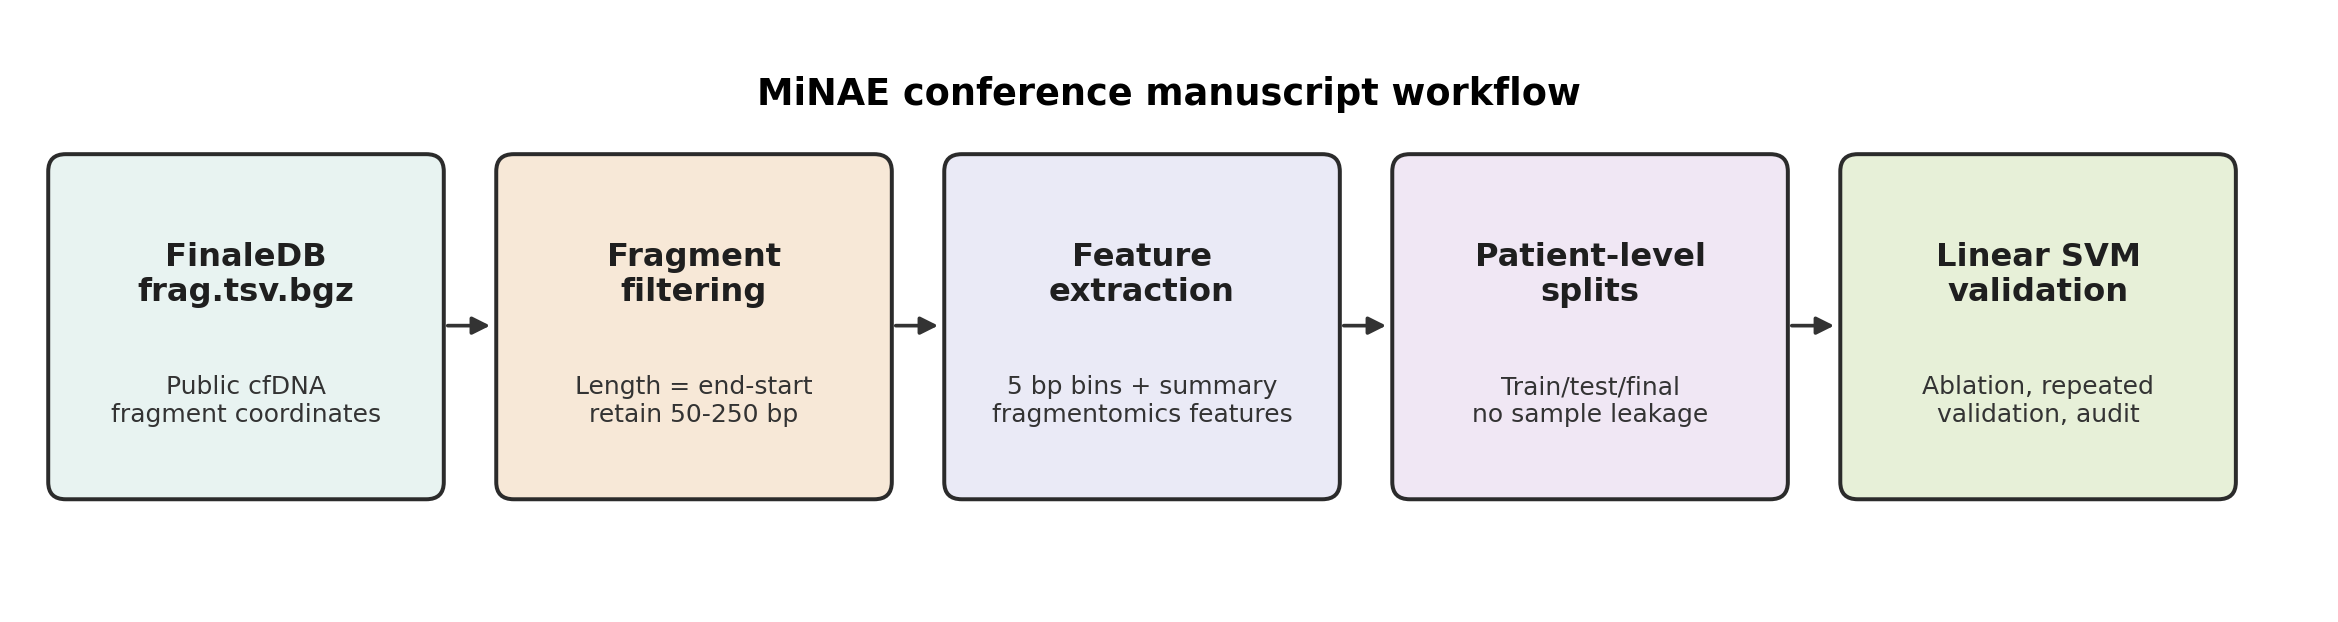
\includegraphics[width=0.93\textwidth]{minae_workflow.png}
\caption{Overview of the MiNAE fragmentomics pipeline. Public FinaleDB fragment-coordinate files are converted into filtered fragment lengths, summarized into normalized feature vectors, split at the patient level, and evaluated with ablation, repeated validation, and statistical audit experiments.}
\label{fig:workflow}
\end{figure*}

\subsection{Global Fragmentomics Features}
Global features were calculated across the whole genome. Fragment lengths from 50 to 250 bp were binned into 5 bp intervals and normalized to create a fragment-size distribution vector. Additional summary features included short-fragment fraction, nucleosome-peak fraction, long-fragment fraction, mean length, median length, interquartile range, skewness, and entropy.

All frequency-bin features were normalized within sample so that the model primarily saw relative fragment-size architecture rather than total fragment abundance. Summary statistics were computed from the filtered fragment-length distribution. Feature extraction was completed before patient-level splitting, but all supervised preprocessing steps, including feature selection and scaling, were fit only inside the training data for each validation run.

\subsection{Dual-Reference Fusion}
FinaleDB provides alignments against both hg19 and hg38 \cite{zheng2021finaledb}. MiNAE evaluated whether reference-sensitive fragmentomic variation added predictive signal by constructing a dual-reference feature vector:
\begin{equation}
    x_{\mathrm{fusion}} = [x_{\mathrm{hg38}}, x_{\mathrm{hg19}}, x_{\mathrm{hg38}} - x_{\mathrm{hg19}}].
\end{equation}
The two reference builds were never treated as separate samples; they were merged into a single row per patient.

\subsection{Chromosome-Targeted Features}
A chromosome-targeted feature strategy was also tested. The targeted groups were gain-associated chromosomes 1 and 8, loss-associated chromosomes 4 and 16, and control chromosomes 2 and 3. These groups were selected as a hypothesis-driven approximation of HCC-relevant copy-number structure. The goal was not to infer copy number directly, but to test whether localized fragment-size distributions improved classification over global profiles.

\section{Modeling and Validation}
\subsection{Classifier}
The primary model family used a linear support vector machine (SVM) with standardization and univariate feature selection:
\begin{equation}
    \mathrm{StandardScaler} \rightarrow \mathrm{SelectKBest} \rightarrow \mathrm{LinearSVM}.
\end{equation}
A linear model was selected because the dataset has many engineered features relative to the number of patients. In small-sample biomedical settings, complex nonlinear models can overfit technical or sampling noise. Linear SVMs provide a more constrained decision boundary while remaining effective for high-dimensional feature spaces \cite{cortes1995support}. Models were implemented using standard Python machine learning tooling \cite{pedregosa2011scikit}.

\subsection{Leakage Prevention and Thresholding}
The main leakage risk in this project is that the same biological sample may appear as both hg19 and hg38 files. MiNAE therefore groups samples by patient/sample identifier before splitting and merges reference builds into a single row when dual-reference features are used. This prevents the model from seeing one genome-build representation of a patient during training and another representation of the same patient during validation.

For each candidate model, feature selection and scaling were fit on the training set only. Decision thresholds were chosen using the test set, not the final validation set. The final validation set was used only once for the locked reported metrics. This separation is important because tuning thresholds or feature counts on the final validation set would overestimate clinical performance.

\subsection{Validation Design}
The main split design used independent patient-level train, test, and final validation sets. The test set was used for model and threshold selection. The final validation set was kept untouched until the selected model was evaluated. The locked split contained 96 training patients, 40 test patients, and 40 final validation patients. The final validation set was balanced with 20 HCC cases and 20 controls.

To test robustness beyond a single split, the split procedure was repeated 100 times with random patient-level partitions. Metrics included ROC-AUC, PR-AUC, accuracy, balanced accuracy, sensitivity, specificity, precision, and F1-score.

Sensitivity was treated as the fraction of HCC cases correctly detected, while specificity was treated as the fraction of chronic liver disease controls correctly rejected. Precision was included because a surveillance biomarker must avoid generating large numbers of false alarms in high-risk populations. Balanced accuracy was reported because it remains interpretable under class imbalance, although the locked final validation set was balanced.

\subsection{Statistical Audit}
Two additional audits were performed. First, a permutation test shuffled training labels and estimated whether the observed final-validation AUC exceeded the null distribution. Second, a technical-feature negative control used only fragment-count-derived features to test whether non-biological technical signal could predict disease labels.

The permutation p-value was calculated as the fraction of shuffled-label AUC values greater than or equal to the observed AUC, with a small-sample correction:
\begin{equation}
    p = \frac{1 + \#(AUC_{\mathrm{perm}} \geq AUC_{\mathrm{obs}})}{1 + N_{\mathrm{perm}}}.
\end{equation}
This test evaluates whether the model exceeds a random-label null distribution, but it does not prove that all learned signal is biological. For that reason, the technical negative control was treated as a separate and necessary audit.

\section{Results}
\subsection{Single Held-Out Validation and Ablation}
Table \ref{tab:ablation} shows the final validation performance for five feature strategies. The strongest single split result came from dual-reference global fusion, which achieved ROC-AUC 0.900, accuracy 0.875, sensitivity 0.850, specificity 0.900, precision 0.895, and F1-score 0.872. Chromosome-targeted fusion achieved similar accuracy and specificity with ROC-AUC 0.890. Combining global and chromosome-targeted features reduced performance, suggesting that increasing feature dimensionality can worsen overfitting in this small cohort.

\begin{table*}[t]
\centering
\caption{Locked final-validation ablation results.}
\label{tab:ablation}
\begin{tabular}{lrrrrrr}
\toprule
Feature strategy & ROC-AUC & Accuracy & Sensitivity & Specificity & Precision & F1 \\
\midrule
hg38 global & 0.828 & 0.750 & 0.750 & 0.750 & 0.750 & 0.750 \\
hg19 global & 0.838 & 0.725 & 0.700 & 0.750 & 0.737 & 0.718 \\
Dual-reference global fusion & 0.900 & 0.875 & 0.850 & 0.900 & 0.895 & 0.872 \\
Chromosome-targeted fusion & 0.890 & 0.875 & 0.850 & 0.900 & 0.895 & 0.872 \\
Global plus chromosome fusion & 0.869 & 0.725 & 0.600 & 0.850 & 0.800 & 0.686 \\
\bottomrule
\end{tabular}
\end{table*}

\begin{figure}[t]
\centering
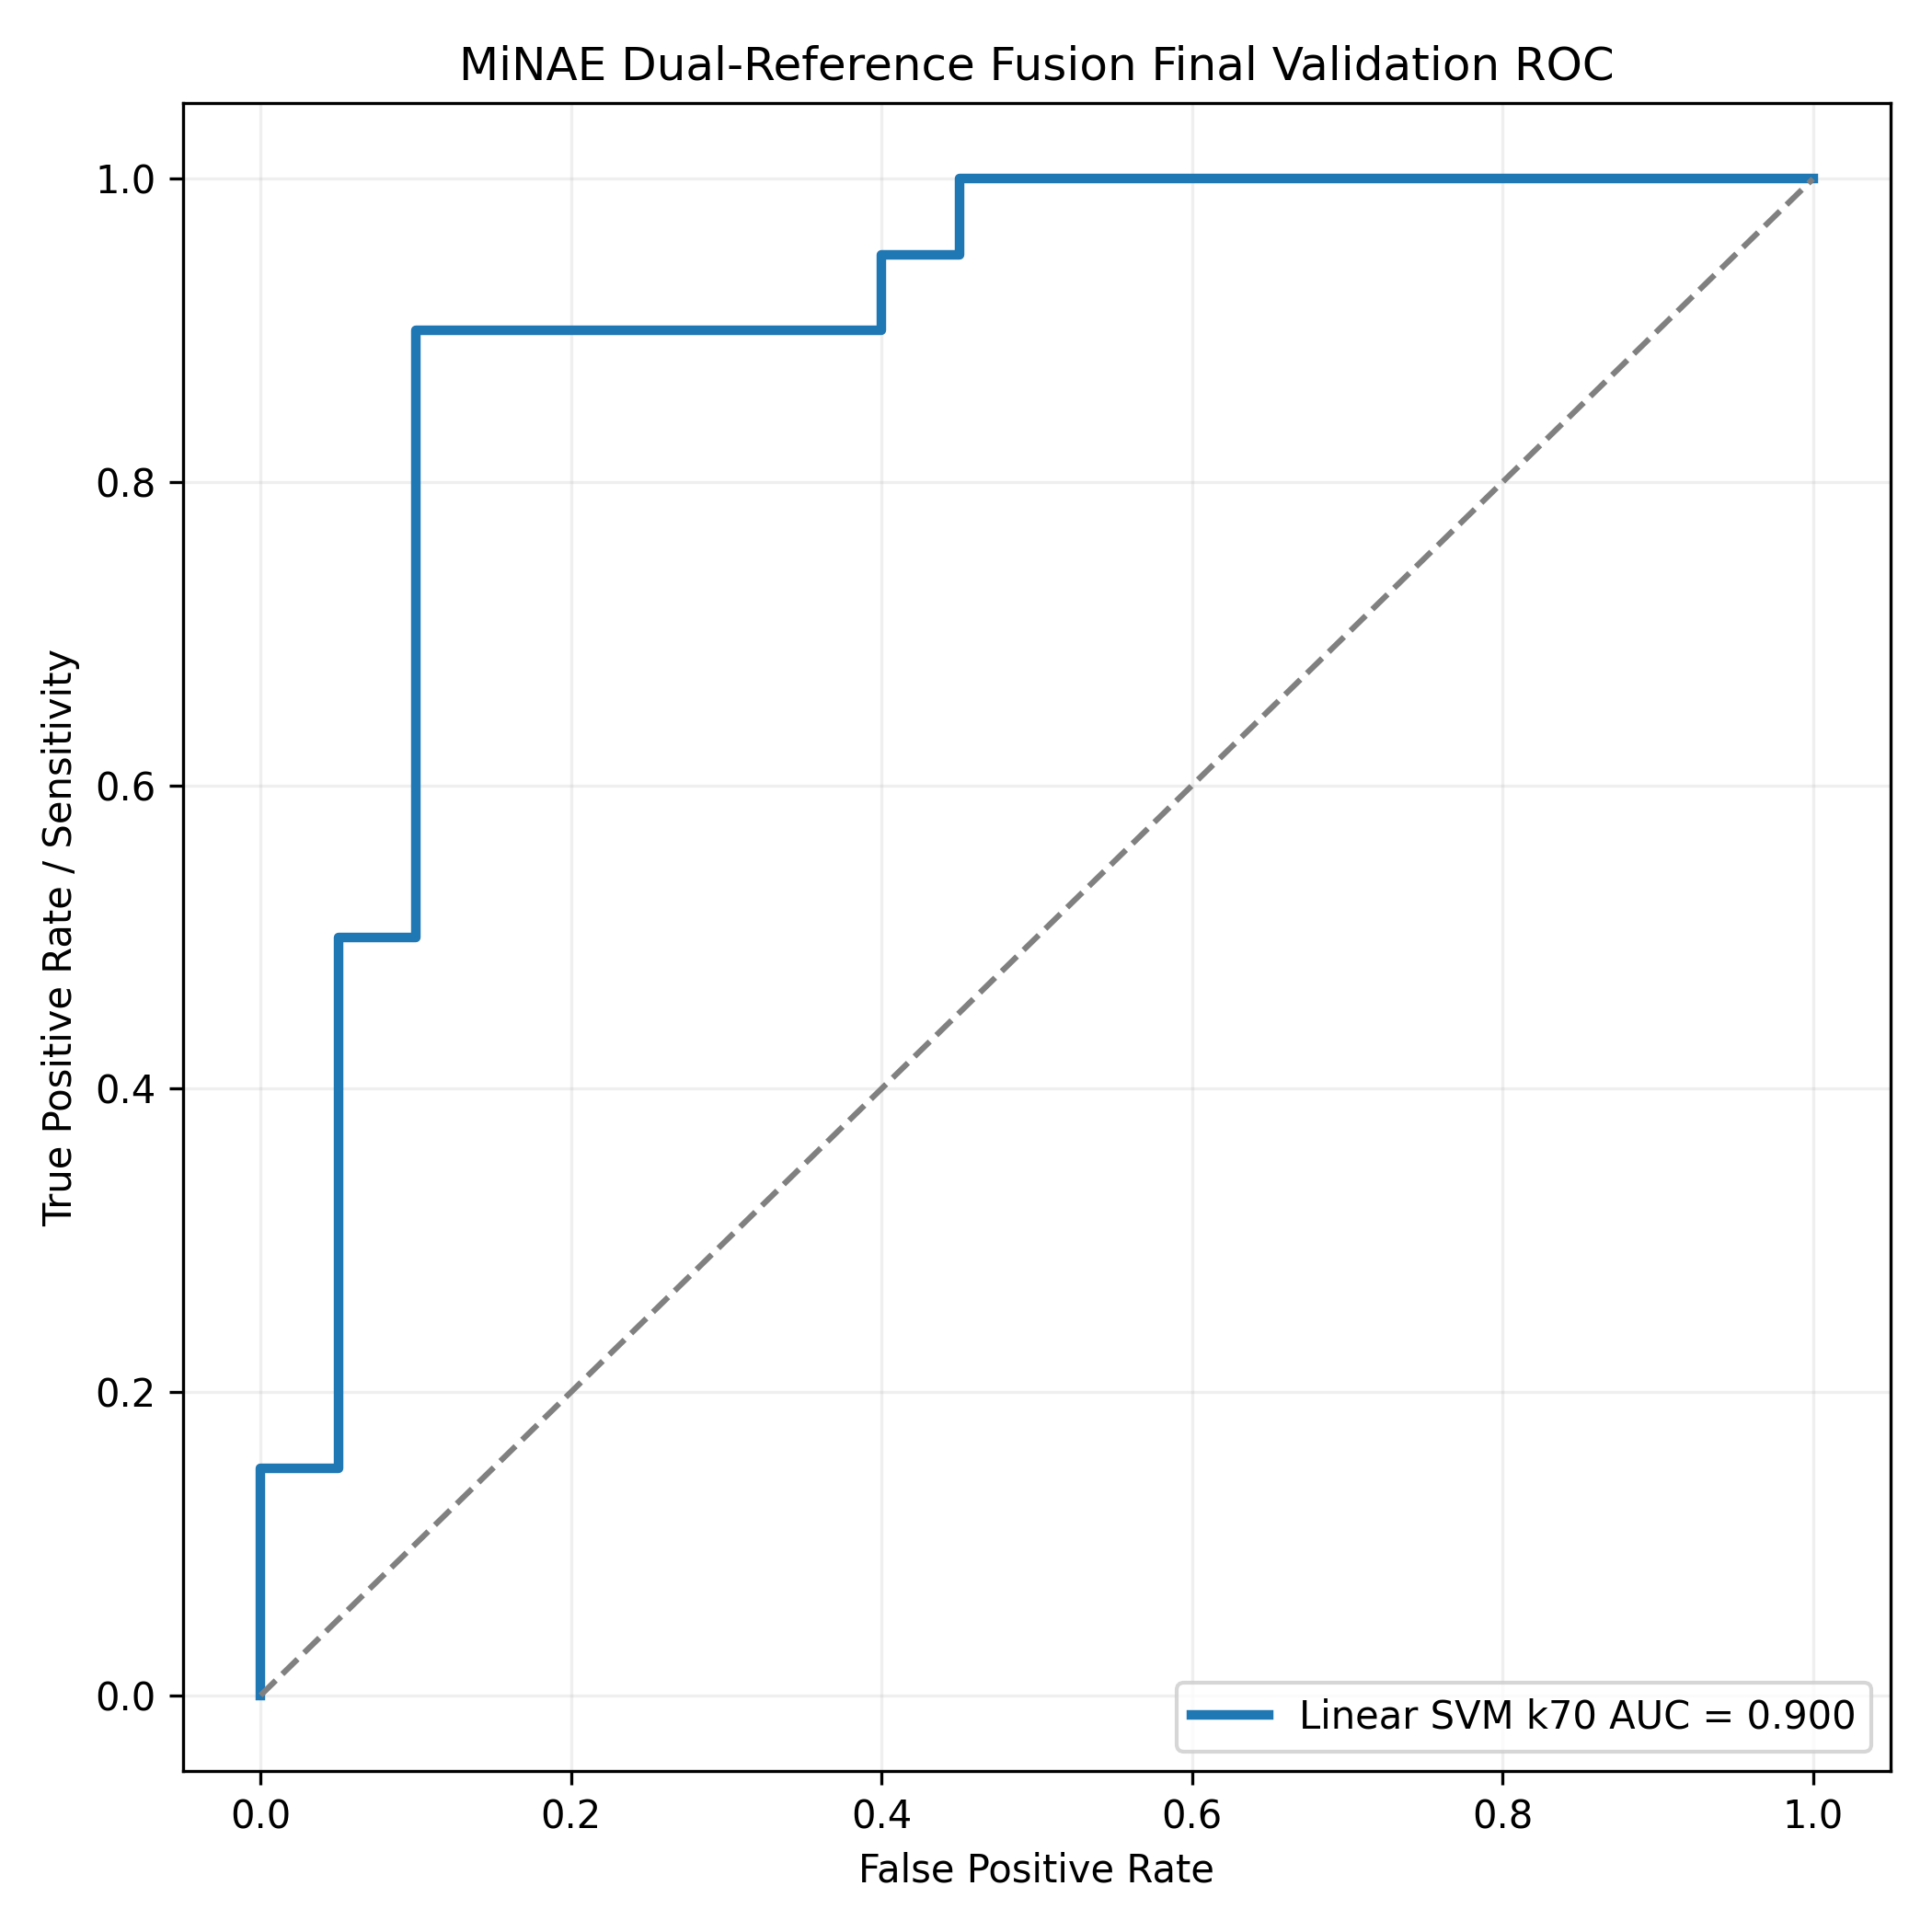
\includegraphics[width=\columnwidth]{final_validation_roc.png}
\caption{Final validation ROC curve for the dual-reference global fusion model. The selected linear SVM achieved ROC-AUC 0.900 on the locked final validation split.}
\label{fig:roc}
\end{figure}

\subsection{Repeated Held-Out Validation}
Table \ref{tab:repeated} reports performance across 100 repeated validations. This experiment changed the interpretation of the single-split results. Although dual-reference fusion performed best in the locked split, hg38 global fragmentomics was the most stable strategy across repeated random splits, with mean ROC-AUC 0.889 and mean accuracy 0.816. This suggests that standard global fragment-size architecture contains robust signal, while more complex feature combinations may be more split-sensitive.

\begin{table*}[t]
\centering
\caption{Repeated held-out validation across 100 patient-level splits.}
\label{tab:repeated}
\begin{tabular}{lrrrrrr}
\toprule
Strategy & Mean ROC-AUC & SD & Mean Acc. & Mean Sens. & Mean Spec. & Mean Prec. \\
\midrule
hg38 global & 0.889 & 0.049 & 0.816 & 0.762 & 0.869 & 0.873 \\
hg19 global & 0.886 & 0.048 & 0.809 & 0.755 & 0.863 & 0.864 \\
Chromosome fusion & 0.872 & 0.052 & 0.761 & 0.727 & 0.795 & 0.806 \\
Dual global fusion & 0.868 & 0.050 & 0.766 & 0.737 & 0.795 & 0.804 \\
Global plus chromosome & 0.847 & 0.057 & 0.751 & 0.698 & 0.805 & 0.798 \\
\bottomrule
\end{tabular}
\end{table*}

\begin{figure}[t]
\centering
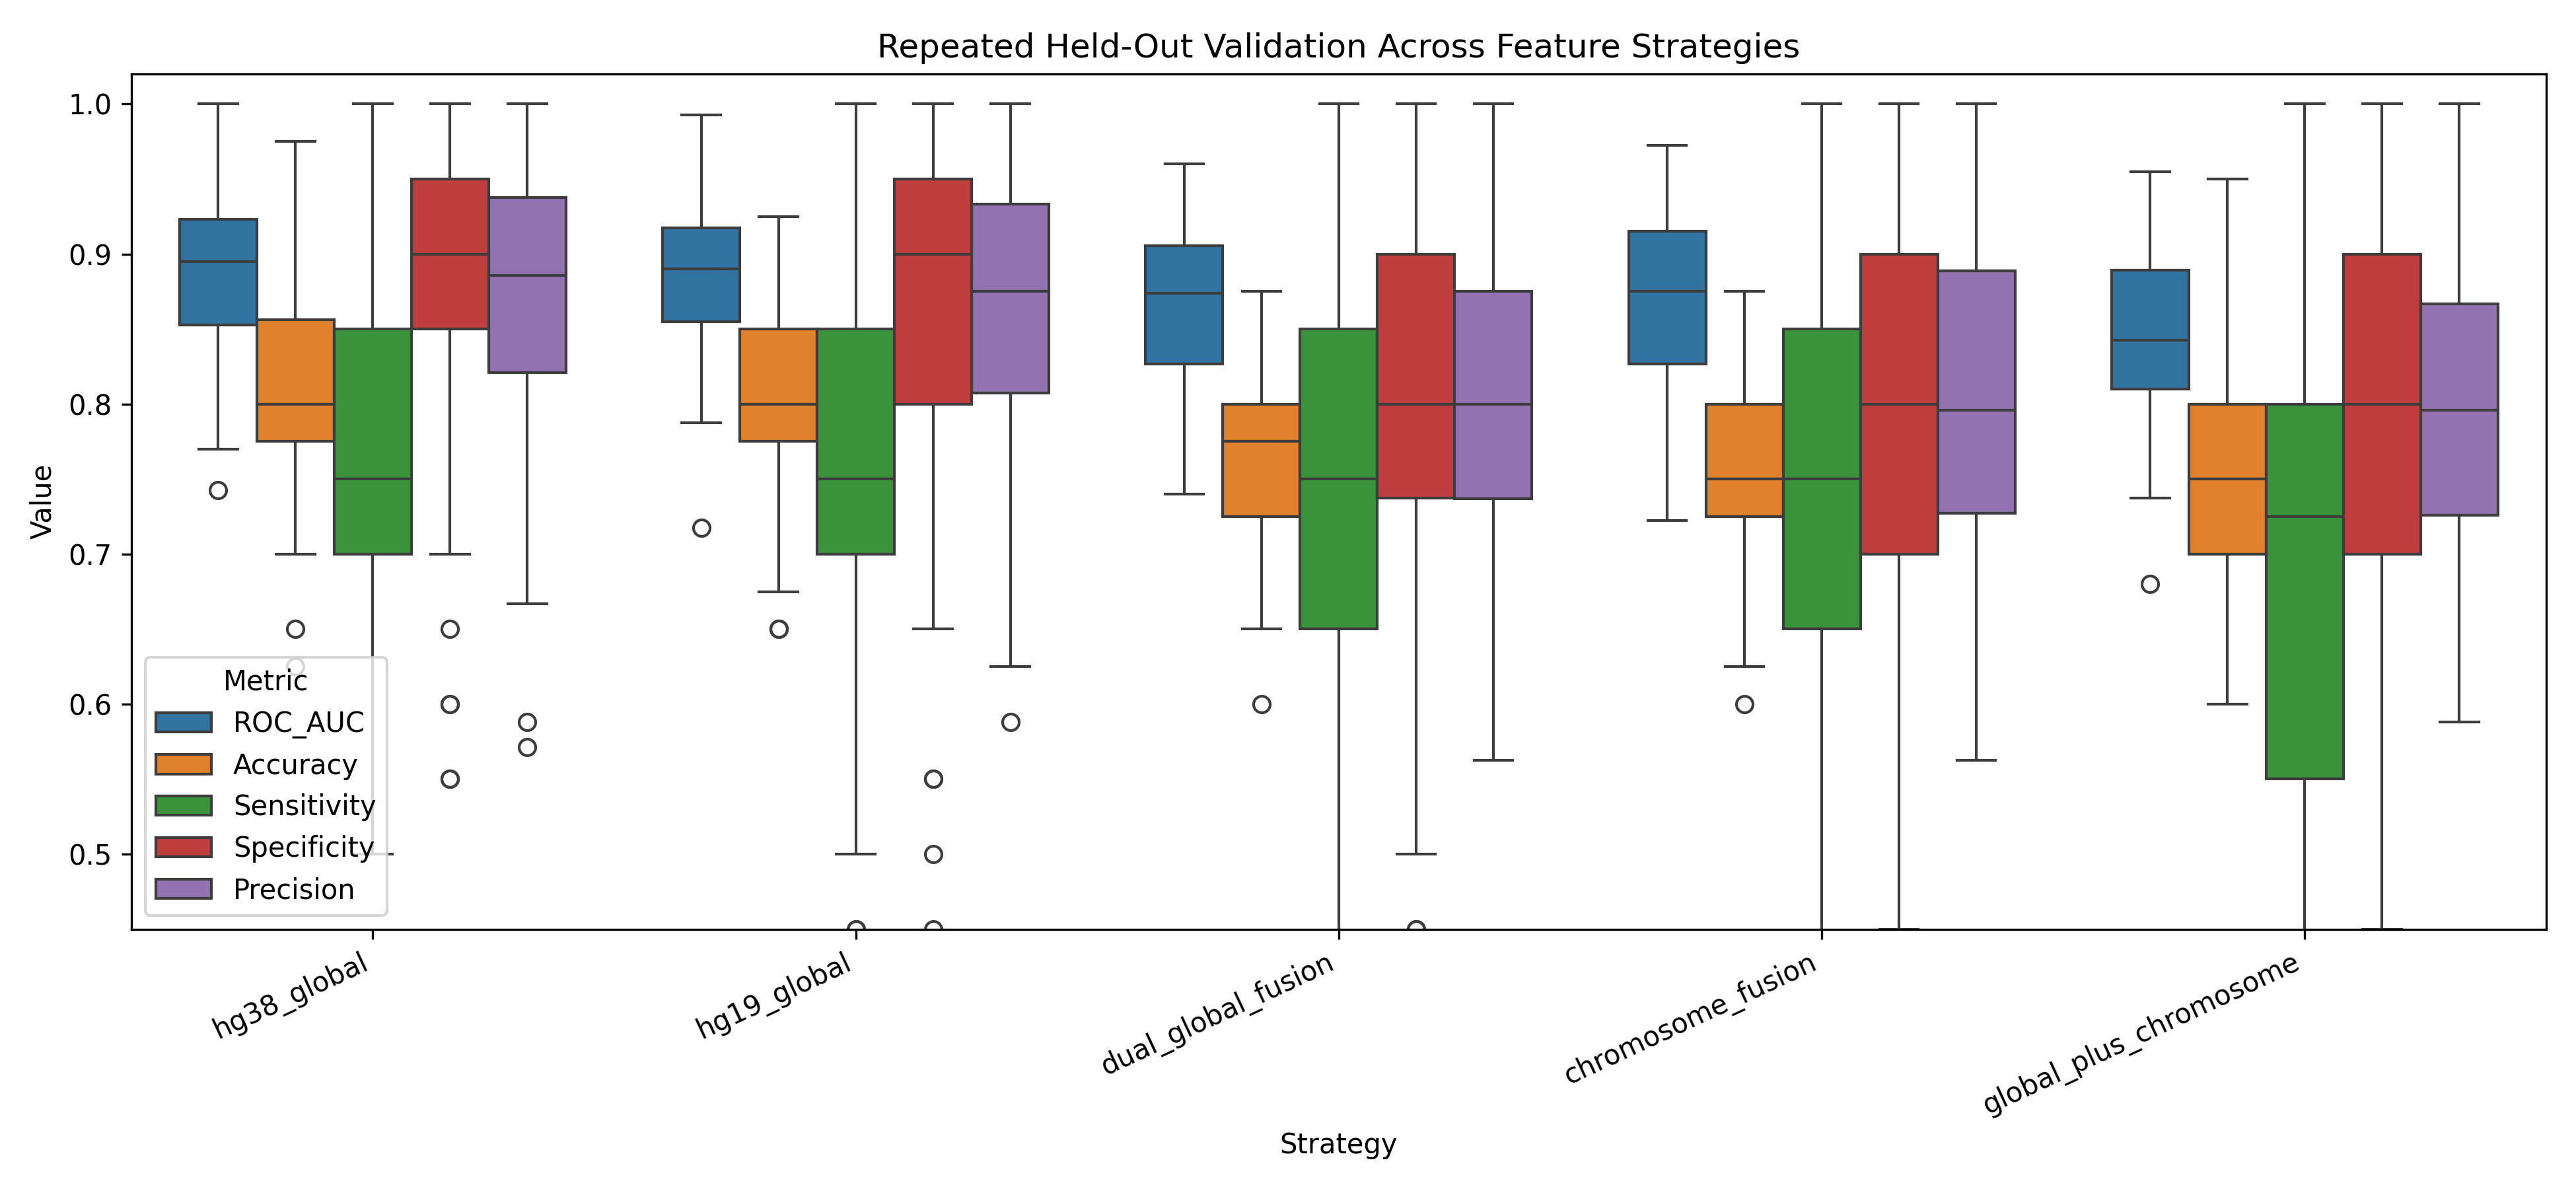
\includegraphics[width=\columnwidth]{repeated_validation_boxplots.png}
\caption{Repeated-validation metric distributions across 100 random patient-level splits. The repeated experiment provides a more conservative estimate than a single split and identifies hg38 global fragmentomics as the most stable strategy in this dataset.}
\label{fig:repeated}
\end{figure}

\subsection{Permutation Test and Negative Control}
The observed final-validation decision-score ROC-AUC was 0.925 in the permutation audit, with permutation p = 0.002. This supports that the observed classification signal is unlikely under random training labels. However, the technical-feature negative control achieved ROC-AUC 0.835, accuracy 0.700, sensitivity 0.400, and specificity 1.000. This is an important caveat: technical covariates or sequencing-depth-related artifacts may be partially associated with class labels in the public data.

Error analysis on the locked final validation set showed 35 correct classifications out of 40 patients. Errors included two false positives among chronic liver disease controls and three false negatives among HCC cases. Specifically, the model made one false positive among cirrhosis controls, one false positive among hepatitis B controls, and three false negatives among liver cancer cases.

\begin{table}[t]
\centering
\caption{Statistical audit and final-validation error summary.}
\label{tab:audit}
\begin{tabular}{lrr}
\toprule
Audit result & Value & Interpretation \\
\midrule
Observed audit ROC-AUC & 0.925 & Non-random signal \\
Permutation p-value & 0.002 & Significant \\
Technical-control ROC-AUC & 0.835 & Confounding risk \\
Final correct / total & 35 / 40 & 87.5\% accuracy \\
False positives & 2 & Control errors \\
False negatives & 3 & Missed HCC cases \\
\bottomrule
\end{tabular}
\end{table}

\begin{figure}[t]
\centering
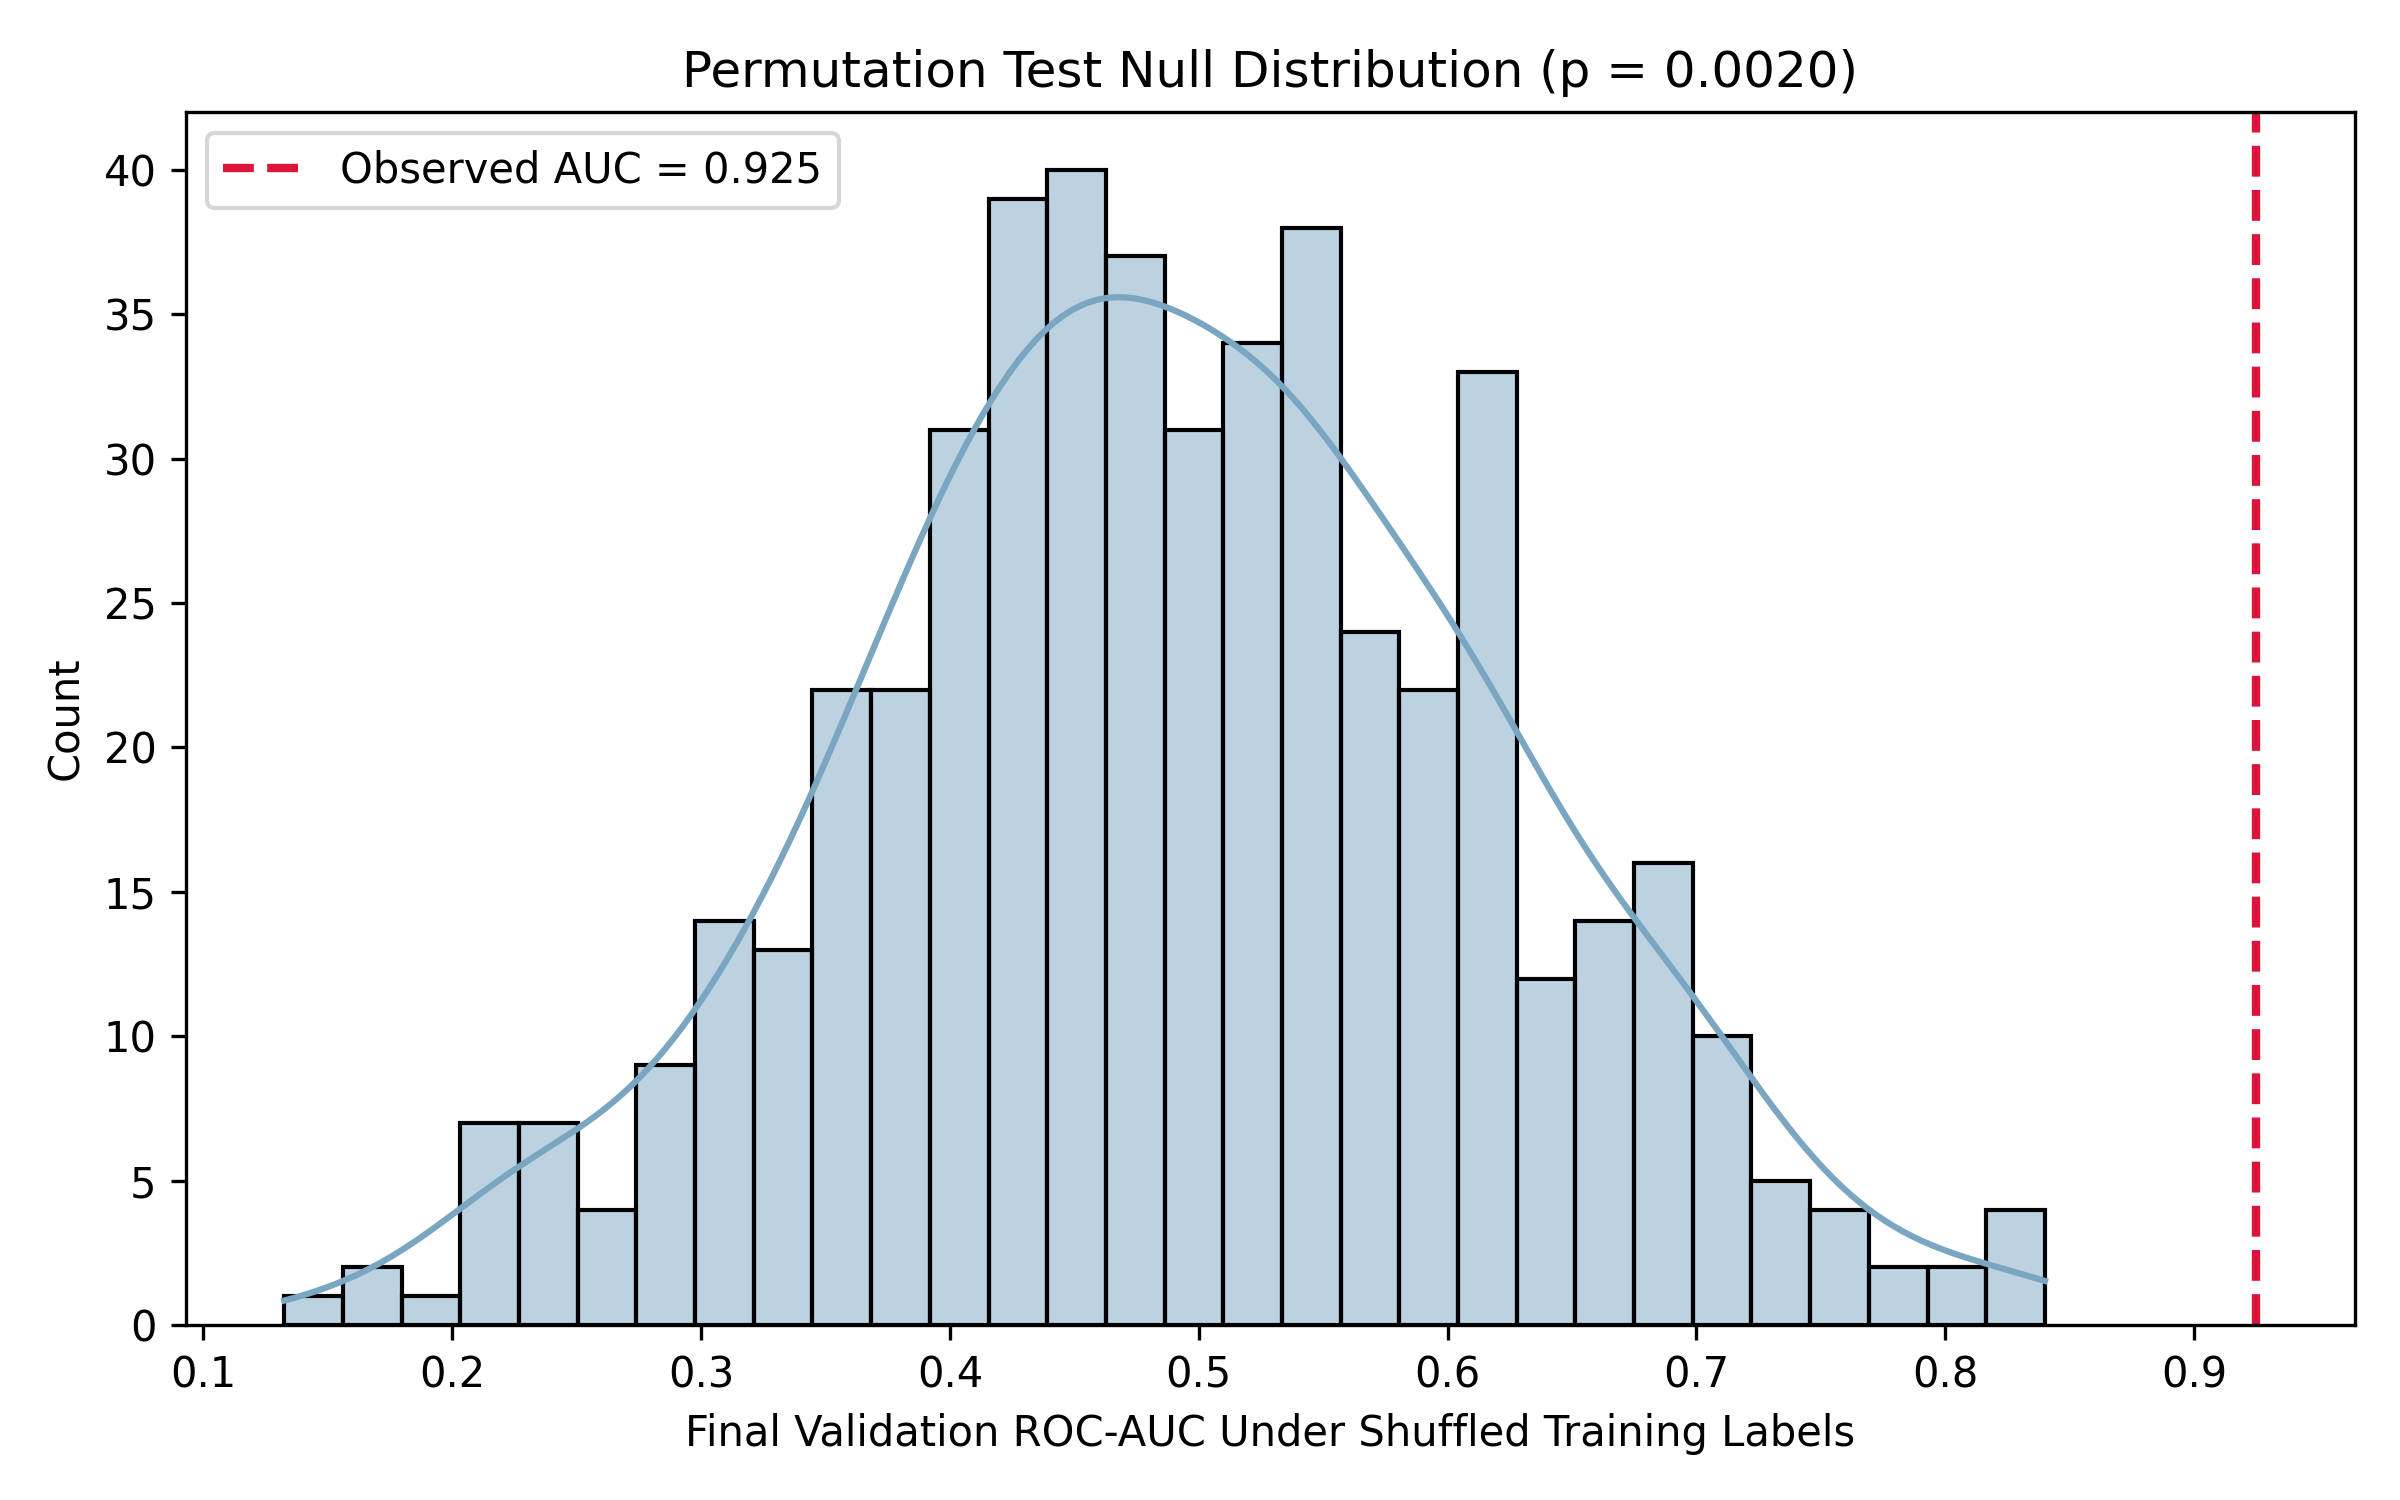
\includegraphics[width=\columnwidth]{permutation_test.png}
\caption{Permutation-test null distribution for final-validation ROC-AUC. The observed model exceeded the shuffled-label null distribution, supporting non-random signal while not resolving possible batch effects.}
\label{fig:permutation}
\end{figure}

\subsection{External Replication and Benchmark}
The Annapragada external fragment-length audit trained on the repository Discovery split and evaluated on its Validation split. Fragmentomics alone achieved ROC-AUC 0.891, accuracy 0.822, sensitivity 0.729, specificity 0.896, and permutation p = 0.003 for advanced fibrosis/cirrhosis versus non-cirrhotic controls. Bootstrap confidence intervals for fragmentomics ROC-AUC were 0.842 to 0.935. However, technical covariates alone achieved ROC-AUC 0.998, and residualizing fragment-length features against technical covariates reduced ROC-AUC to 0.799. This indicates that fragment-length architecture replicated externally, but technical or cohort structure remains a major confounding concern.

Source-level holdout was more conservative. The only held-out source with enough samples from both classes, INCAP, produced ROC-AUC 0.699, suggesting that model performance weakens under stricter cohort-shift conditions. In the Foda supplementary benchmark, the published DELFI-surveillance score achieved ROC-AUC 0.900 for HCC versus cirrhosis/HBV/HCV controls and ROC-AUC 0.889 for HCC versus cirrhosis alone. These results contextualize the clinical HCC task but are not MiNAE predictions.

\begin{table*}[t]
\centering
\caption{External replication and benchmark audit. Annapragada results use external fragment-length tables; Foda results use published DELFI-surveillance scores, not MiNAE predictions.}
\label{tab:external}
\begin{tabular}{lrrrrr}
\toprule
External analysis & N & ROC-AUC & Accuracy & Sensitivity & Specificity \\
\midrule
Annapragada fragmentomics, Discovery-to-Validation & 191 & 0.891 & 0.822 & 0.729 & 0.896 \\
Annapragada technical covariates only & 191 & 0.998 & 0.921 & 0.835 & 0.991 \\
Annapragada residualized fragmentomics & 191 & 0.799 & 0.733 & 0.624 & 0.821 \\
Annapragada held-out INCAP source & 66 & 0.699 & 0.667 & 0.771 & 0.389 \\
Foda DELFI score, HCC vs cirrhosis/HBV/HCV & 208 & 0.900 & 0.851 & 0.787 & 0.887 \\
Foda DELFI score, HCC vs cirrhosis only & 153 & 0.889 & 0.830 & 0.787 & 0.872 \\
\bottomrule
\end{tabular}
\end{table*}

\section{Discussion}
MiNAE supports the hypothesis that cfDNA fragment-size architecture contains signal for distinguishing HCC from chronic liver disease controls. The strongest single held-out validation result reached ROC-AUC 0.900, but the repeated-validation experiment is the more important result for scientific interpretation. Across 100 random splits, hg38 global fragmentomics was most stable, suggesting that the core fragment-size distribution signal is more reliable than the more elaborate dual-reference or combined feature strategies in the present cohort.

The ablation study provides two useful lessons. First, dual-reference and chromosome-targeted features can produce strong held-out performance, indicating that both reference-sensitive and chromosome-localized fragmentomics deserve further investigation. Second, adding more features did not automatically improve the model. The global-plus-chromosome strategy performed worse than simpler strategies, consistent with overfitting in a small-sample, high-feature setting.

The technical negative control is a central limitation and should be viewed as a strength of the audit rather than a failure of the project. It shows that public retrospective cfDNA datasets can contain class-associated technical structure. The external Annapragada analysis reinforced this concern: fragmentomics replicated with strong Discovery-to-Validation performance, but technical covariates alone were highly predictive and source-level holdout was weaker. Therefore, the current results should be interpreted as evidence for a promising fragmentomic signal, not as proof of a deployable clinical diagnostic. Future studies should include independent HCC fragment-length validation, study-level splits, explicit sequencing-depth and batch adjustment, and comparison against clinical variables such as AFP, ultrasound findings, tumor stage, cirrhosis severity, and hepatitis status.

The difference between the locked final split and repeated validation is also informative. The locked split suggests that dual-reference fusion can be useful, but repeated validation suggests that the simpler hg38 global model is more stable on average. A less cautious paper might report only the best split and overstate the dual-reference result. MiNAE instead reports both results and treats split sensitivity as part of the finding. For biomedical machine learning, this is important because reproducibility depends on the stability of the signal, not only on the strongest observed metric.

\subsection{Implications for Public-Data Biomarker Studies}
The results highlight a broader lesson for public biomedical machine learning. A high single-split AUC is insufficient when the dataset is small and samples may share hidden technical structure. The repeated-validation results provide a more conservative estimate of expected performance, while the negative control reveals whether apparently biological signal may be mixed with technical artifacts. For public cfDNA data, these audits are especially important because sample acquisition, sequencing protocols, and study origin can be difficult to reconstruct from de-identified files.

MiNAE therefore contributes less as a new classifier architecture and more as a validation pattern: build biologically motivated fragmentomic features, avoid patient leakage, compare simpler and more complex feature strategies, repeat validation many times, and explicitly test technical shortcuts. This framework can be reused for other public cfDNA classification tasks where raw data access is limited but coordinate-level fragment information is available.

\section{Reproducibility and Availability}
All experiments were designed to be reproducible from public FinaleDB fragment-coordinate files and deterministic patient-level split definitions. The analysis pipeline produces intermediate feature matrices, split files, final predictions, ablation tables, ROC curves, repeated-validation summaries, and statistical-audit outputs. During double-blind review, identifying repository links are omitted. If accepted, the code, processed feature tables, and exact split manifests should be released in a public repository so that other researchers can reproduce the reported results and test alternative feature strategies.

The most important reproducibility objects are: the sample manifest mapping disease labels to FinaleDB files, the patient-level train/test/final validation split, the normalized feature matrices for each feature strategy, the model-selection table from the test set, and the final-validation prediction table. Reporting these artifacts reduces ambiguity about which samples were used and prevents accidental leakage when extending the work.

\section{Limitations}
This study has several limitations. The data are public and retrospective rather than prospectively collected. The final validation set is small, and no independent external HCC fragment-length cohort was available. Tumor stage, AFP values, ultrasound results, liver disease severity, and treatment status were not consistently available, preventing early-stage-specific or clinically adjusted analyses. Although patient-level splitting prevented leakage across reference builds, study-level confounding may remain. The negative-control model showed that technical features can predict labels above chance, and the external Annapragada audit confirmed that technical covariates can dominate some public fragmentomics tasks, requiring more rigorous batch-effect analysis before clinical claims can be made.

The chromosome-targeted analysis is also exploratory. Chromosomes 1, 4, 8, and 16 were selected as biologically motivated HCC-associated regions, but this study did not directly measure tumor copy-number alterations or local chromatin states. Future work should connect chromosome-localized fragmentomics to matched tumor biology, cell-type-of-origin estimates, or independent epigenomic annotations.

\section{Conclusion}
MiNAE is a reproducible public-data framework for evaluating cfDNA fragmentomics in HCC detection. In a patient-level held-out validation design, fragment-size features distinguished HCC from cirrhosis and hepatitis B controls with strong but preliminary performance. External liver-disease fragment-length replication supported the presence of fragmentomic signal but also demonstrated substantial technical confounding. The most defensible conclusion is that cfDNA fragment-size architecture carries measurable disease-associated signal in public data, and that rigorous ablation, repeated validation, external replication, and technical audits are necessary before translating such models toward clinical use.

\section*{Acknowledgment}
Acknowledgments are omitted for double-blind review.

\bibliographystyle{IEEEtran}
\bibliography{references}

\end{document}
